\documentclass{article}
\usepackage{graphicx}
\usepackage{amsmath}
\usepackage{pgfplots}
\usepackage{siunitx}
\usepackage{cancel}
\usepackage{enumitem}
\usepackage{txfonts}

\pgfplotsset{compat=1.18}

\usepackage[a4paper, top=1cm, bottom=2cm, left=2cm, right=2cm, includehead, includefoot]{geometry}

\begin{document}

\noindent
Physics 4A - Classical Mechanics \hfill Prof. Roger King

\noindent\rule{\textwidth}{0.4pt}

\begin{center}
    \textbf{\LARGE Homework 2} \\
    \vspace{12pt}
    \large Aaron W. Tarajos \\
    \textit{\today}
\end{center}

\noindent\rule{\textwidth}{0.4pt}

\section*{Problem 1}
In the graph below, is there any time, or time interval, for which the following hold? (a)
$v = 0,\ a = 0$; (b) $v = 0,\ a \ne 0$; (c) $v \ne 0, a = 0$; (d) $v > 0,\ a > 0$; (e) $v > 0,\ a < 0$;
(f) $v < 0,\ a < 0$; (g) $v < 0,\ a > 0$.

\begin{figure}[ht]
    \centering
    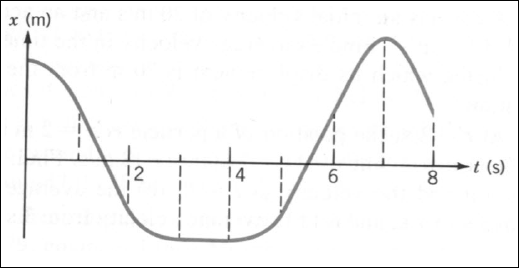
\includegraphics[scale=0.5]{graph-1.png}
\end{figure}

\subsection*{Solution}
(a) $v = 0,\ a = 0$. From $t = 3$ to $t = 4$, the slope of $x(t)$ is zero, so $v = 0$. The slope of $v(t)$ is also zero, so $a = 0$.\\
(b) $v = 0,\ a \ne 0$. At $t = 7$, the slope of $x(t)$ is zero, so $v = 0$. However, $a \ne 0$ since $x(t)$ has positive slope before and negative slope after $t = 7$, meaning the velocity changes from positive to negative, and thus $a \ne 0$.\\
(c) $v \ne 0,\ a = 0$. From $t = 1$ to $t = 2$ and $t = 5$ to $t = 6$, $v(t)$ is constant (negative from $1$ to $2$, positive from $5$ to $6$), so $v \ne 0$ and $a = 0$ in both intervals.\\
(d) $v > 0,\ a > 0$. From $t = 4$ to $t = 5$, the slope of $x(t)$ is positive and increasing, so $v > 0$ and $a > 0$.\\
(e) $v > 0,\ a < 0$. From $t = 6$ to $t = 7$, $x(t)$ has positive slope, so $v > 0$. The slope is decreasing, so $a < 0$.\\
(f) $v < 0,\ a < 0$. From $t = 0$ to $t = 1$ and $t = 7$ to $t = 8$, $x(t)$ has negative slope and decreasing, so $v < 0$ and $a < 0$ in both intervals.\\
(g) $v < 0,\ a > 0$. From $t = 2$ to $t = 3$, $x(t)$ has negative slope, so $v < 0$. The slope is increasing, so $a > 0$.\\

\section*{Problem 2}
The figure below shows the $v$ versus $t$ graphs for cars A and B. At $t = 0$ both are at $x = 0$.
Estimate: (a) where and when they meet again; and (b) their velocities when they meet.

\begin{figure}[ht]
    \centering
    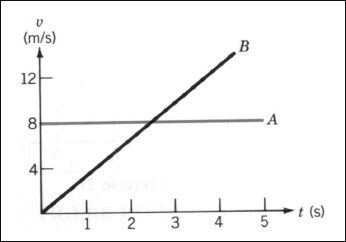
\includegraphics[scale=0.5]{graph-2.png}
\end{figure}

\subsection*{Solution}
To find when and where the cars meet again after $t = 0$, we must find when $\Delta x$ is equal for both cars. Car A has constant velocity which means that $\Delta x$ is given by;

\[
	\Delta x = v_A t
\]
where $v_A$ is the velocity of Car A. Also, we can see that Car B has constant acceleration which means that $\Delta x$ is given by;
\[
	\Delta x = v_{0B} t + \frac{1}{2} a t^2
\]
where $v_{0B}$ is the initial velocity of car B. We set these equations equal to eachother and re-arrange it to solve for time.
\begin{align*}
	v_A t &= v_{0B} t + \frac{1}{2} a t^2 \\
	v_A t &= \left( v_{0B} + \frac{1}{2} a t \right) t \\
	v_A - v_{0B} &= v_{0B} + \frac{1}{2} a t  - v_{0B} \\
	2 \left( v_A - v_{0B} \right) &= \frac{1}{2} a t \cdot 2 \\
	t &= \frac{2 \left( v_A - v_{0B} \right)}{a} \\
\end{align*}
Looking at the graph we can estimate $a$ for car B to be $3\ \unit{\meter\per\second^2}$, then substituting our variables, we find that the cars meet again at;
\[
	\frac{2 \left( 8.00 - 0.00 \right)}{3.00} = \frac{16}{3}\ \unit{\second}
\]
or approximately 5.33 seconds. Then we use the time in one of our original equation for $\Delta x$ and find that the cars meet again at;

\[
	\left( 8 \right) \cdot \left(\frac{16}{3}\right) = \frac{128}{3}\ \unit{\meter}
\]
which is approximately 42.66 meters. Now, we already know that $v_A$ is constant so it will be 8, however, for car B we must use our acceleration estimate $a$ and $t$ to find the velocity.
\begin{align*}
	v_B &= v_{0b} + at \\
	v_B &= 0 + \left( 3 \right) \cdot \left( \frac{16}{3} \right) \\
	v_B &= 16\ \unit{{\meter\per\second}}
\end{align*}

\section*{Problem 3}
A Honda Fit is initially with a speed of 115 km/h. Find its acceleration and the time taken
to stop given that: (a) it brakes to a stop in 64.0 m; (b) it crashes head-on into a barrier and
crumples by 1.00 m.

\subsection*{Solution}
Given that we are missing time, we can use the following equation to solve for acceleration in both circumstances;
\begin{align*}
	v^2 &= 2a \Delta x + v_0^2 \\
	v^2  - v_0^2 &= 2a \Delta x
\end{align*}
\begin{equation}
	a = \frac{v^2  - v_0^2}{2\Delta x}
\end{equation}
and solve for time using
\begin{align*}
	\Delta x &= \frac{v + v_0}{2} t \\
	2 \Delta x &= \left(v + v_0 \right) t \\
\end{align*}
\begin{equation}
	t = \frac{2 \Delta x}{v + v_0}
\end{equation}
We have a unit conversion from km/h to m/s so that we have consistent units for distance and so that the timescale matches the distance units.
\[
	115\ \unit{\kilo\meter\per\hour} \cdot 1000\ \unit{{\meter\per\kilo\meter}} \cdot \frac{1}{3600}\ \unit{\hour\per\second} = 31.944\ \unit{{\meter\per\second}}
\]
Now we subsitute our values into Eq.1 to find that aceleration when braking to a stop is;
\[
	\frac{0 - 31.944^2}{2\left(64.0\right)} = -8.0\ \unit{\meter\per\second^2}
\]
The time elapsed over that distance using Eq.2 is;

\[
	t = \frac{2 \Delta x}{v + v_0}
\]
\[
	\frac{2 (64.0)}{0 + 31.944} = 4.0\ \unit{\second}
\]
For the case where the car is stopped by a pole 1.00 m away. We use the same equations;
\[
	\frac{0-31.944^2}{2(1.00)} = -510.2\ \unit{\meter\per\second^2}
\]
and

\[
	\frac{2(1)}{0 + 31.944} = 0.06\ \unit{\second}
\]

\section*{Problem 4}
An object moves with constant acceleration. At $t = 2.50$ s, the position of the object is
$x = 2.00$ m and its velocity is $v = 4.50$ m/s. At $t = 7.00$ s, $v = -12.0$ m/s. Find: (a) the
position and the velocity at $t = 0$; (b) the average speed from 2.50 s to 7.00 s, and (c) the
average velocity from 2.50 s to 7.00 s.

\subsection*{Solution}
\subsubsection*{Part a:}
We start by finding the acceleration
\begin{align*}
	v &= at + v_0 \\
	v - v_0 &= at \\
	a &= \frac{v - v_0}{t} \\
	\frac{-12.00 - 4.50}{4.50} &= \frac{-16.50}{4.50}\ \unit{\meter\per\second^2}
\end{align*}
Then the velocity at $t=0$ is
\begin{align*}
	v &= at + v_0 \\
	v_0 &= v - at \\
	v_0 &= 4.50 - \left(\frac{-16.50}{4.50}\right) 2.50 \\
	v_0 &= 13.66\ \unit{{\meter\per\second}}
\end{align*}
and the position at $t=0$ is;
\begin{align*}
	x_0 = x - \frac{v + v_0}{2} t \\
	x_0 = 2 - \frac{4.50 + 13.66}{2} 2.50 \\
	x_0 = -20.7
\end{align*}

\subsubsection*{Part b:}
Average speed is the total distance traveled over time which we can derive using our constant acceleration of $3.66$ m/s$^2$.
\begin{align*}
	a &= 3.66\ \unit{\meter\per\second^2} \\
	\int dv &= \int 3.66 \quad dt \\
	v &= 3.66t \\
	\int dx &= \int 3.66t \quad dt \\
		&= \frac{3.66t^2}{2} + 13.66t - 20.7
\end{align*}
which gives us an area of $22.3754$ and therefore an average speed of;
\[
	s_{avg} = \frac{22.3754}{4.5} = 4.97\ \unit{{\meter\per\second}}
\]

\section*{Problem 5}
A ball thrown vertically up from the ground rises to height of 24.0 m. How high would it rise
on the moon if given the same initial speed? The acceleration due to gravity on the moon is one-
sixth that on earth.

\subsection*{Solution}
We need to solve for initial velocity given the information that we have and use it to find the change in position with a different free-fall acceleration.
\begin{align*}
	v^2 &= v_0^2 + 2a \Delta x \\
	v_0^2 & = v^2 - 2a \Delta x \\
	v_0^2 &= (0)^2 -2(-9.8)(24) \\
	v_0 &= \sqrt{470.4}
\end{align*}
Now we substitute the initial velocity into the same equation with the new free-fall acceleration to solve for $\Delta x$.
\begin{align*}
	v^2 &= v_0^2 + 2a \Delta x \\
	v^2 - v_0^2 &= 2a \Delta x \\
	\Delta x &= \frac{v^2 - v_0^2}{2a} \\
	\Delta x &= \frac{(0)^2 - \left( \sqrt{470.4} \right)^2}{2(-1.635)} \\
	\Delta x &= 143.9\ \unit{\meter}
\end{align*}

\section*{Problem 6}
A ball is thrown up from the top of a building 55.0 m high. It rises to a maximum height
of 20.0 m above the roof. (a) When does it land on the ground below? (b) At what velocity
does it land? (c) When is it 20.0 m below the roof?

\subsection*{Solution}
\subsubsection*{Part a:}
We start by finding $v_0$, given that the maximum height of the ball is 20.0 m above the roof. At maximum height, the velocity is zero, so we use the following equation:
\[
	v^2 = v_0^2 + 2a\Delta x
\]
At maximum height, $v = 0$, $a = -9.8\ \unit{\meter\per\second^2}$, and $\Delta x = 20.0\ \unit{\meter}$, so we solve for $v_0$:
\[
	0 = v_0^2 - 2(9.8)(20.0)
\]
\[
	v_0^2 = 392.0
\]
\[
	v_0 = \sqrt{392.0}\ \unit{{\meter\per\second}}
\]
Now that we have $v_0$, we substitute it into
To find the time taken to hit the ground, we use:
\[
	\Delta x = v_0 t + \frac{1}{2} a t^2
\]
to find the time it takes for the ball to hit the ground. The total displacement is $-55.0\ \unit{\meter}$:
\[
	-55.0 = \sqrt{392.0}t + \frac{1}{2}(-9.8)t^2
\]
\[
	-55.0 = \sqrt{392.0}t - 4.9t^2
\]
Using the quadratic formula:
\[
	t = \frac{-(-\sqrt{392.0}) \pm \sqrt{(-\sqrt{392.0})^2 - 4(4.9)(-55.0)}}{2(4.9)}
\]
\[
	t = \frac{19.8 \pm \sqrt{392.0 + 1078.0}}{9.8}
\]
\[
	t = \frac{19.8 \pm \sqrt{1470.0}}{9.8}
\]
\[
	t = \frac{19.8 \pm 38.34}{9.8}
\]
\[
	t = \frac{19.8 + 38.34}{9.8} = 5.93\ \unit{\second}
\]
\subsubsection*{Part b:}
To find the velocity at the moment the ball hits the ground, we use the equation:
\[
	v = v_0 + at
\]
Substituting the known values:
\[
	v = 19.8 + (-9.8)(6.43)
\]
\[
	v = 19.8 - 63.0
\]
\[
	v = -43.2\ \unit{{\meter\per\second}}
\]

\subsubsection*{Part c:}
To find when the ball is 20.0 m below the roof (i.e., at $55.0 - 20.0 = 35.0\ \unit{\meter}$ above the ground), we again use the kinematic equation:
\[
	\Delta x = v_0 t + \frac{1}{2} at^2
\]
where $\Delta x = -20.0\ \unit{\meter}$. Substituting the known values:
\[
	-20.0 = 19.8t + \frac{1}{2}(-9.8)t^2
\]
\[
	-20.0 = 19.8t - 4.9t^2
\]
Using the quadratic formula:
\[
	t = \frac{-(-19.8) \pm \sqrt{(-19.8)^2 - 4(4.9)(-20.0)}}{2(4.9)}
\]
\[
	t = \frac{19.8 \pm \sqrt{392.04 + 392.0}}{9.8}
\]
\[
	t = \frac{19.8 \pm \sqrt{784.04}}{9.8}
\]
\[
	t = \frac{19.8 \pm 28.0}{9.8}
\]
Taking the positive root:
\[
	t = \frac{19.8 + 28.0}{9.8} = \frac{47.8}{9.8} = 4.88\ \unit{\second}
\]
Therefore, the ball is 20.0 m below the roof at $t = 4.88\ \unit{\second}$.


\section*{Problem 7}
From the $v$ versus $t$ graph below, plot the following graphs: (a) $a$ versus $t$; (b) $x$ versus $t$.
(c) What is the average acceleration for the first 6.0 s? (d) What is the instantaneous
acceleration at 2.0 s? Assume $x = 0$ at $t = 0$.

\begin{figure}[ht]
    \centering
    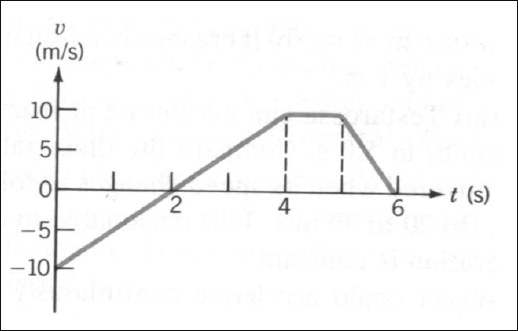
\includegraphics[scale=0.5]{graph-3.png}
\end{figure}

\pagebreak
\subsection*{Solution}
\begin{figure}[!ht]
    \centering
    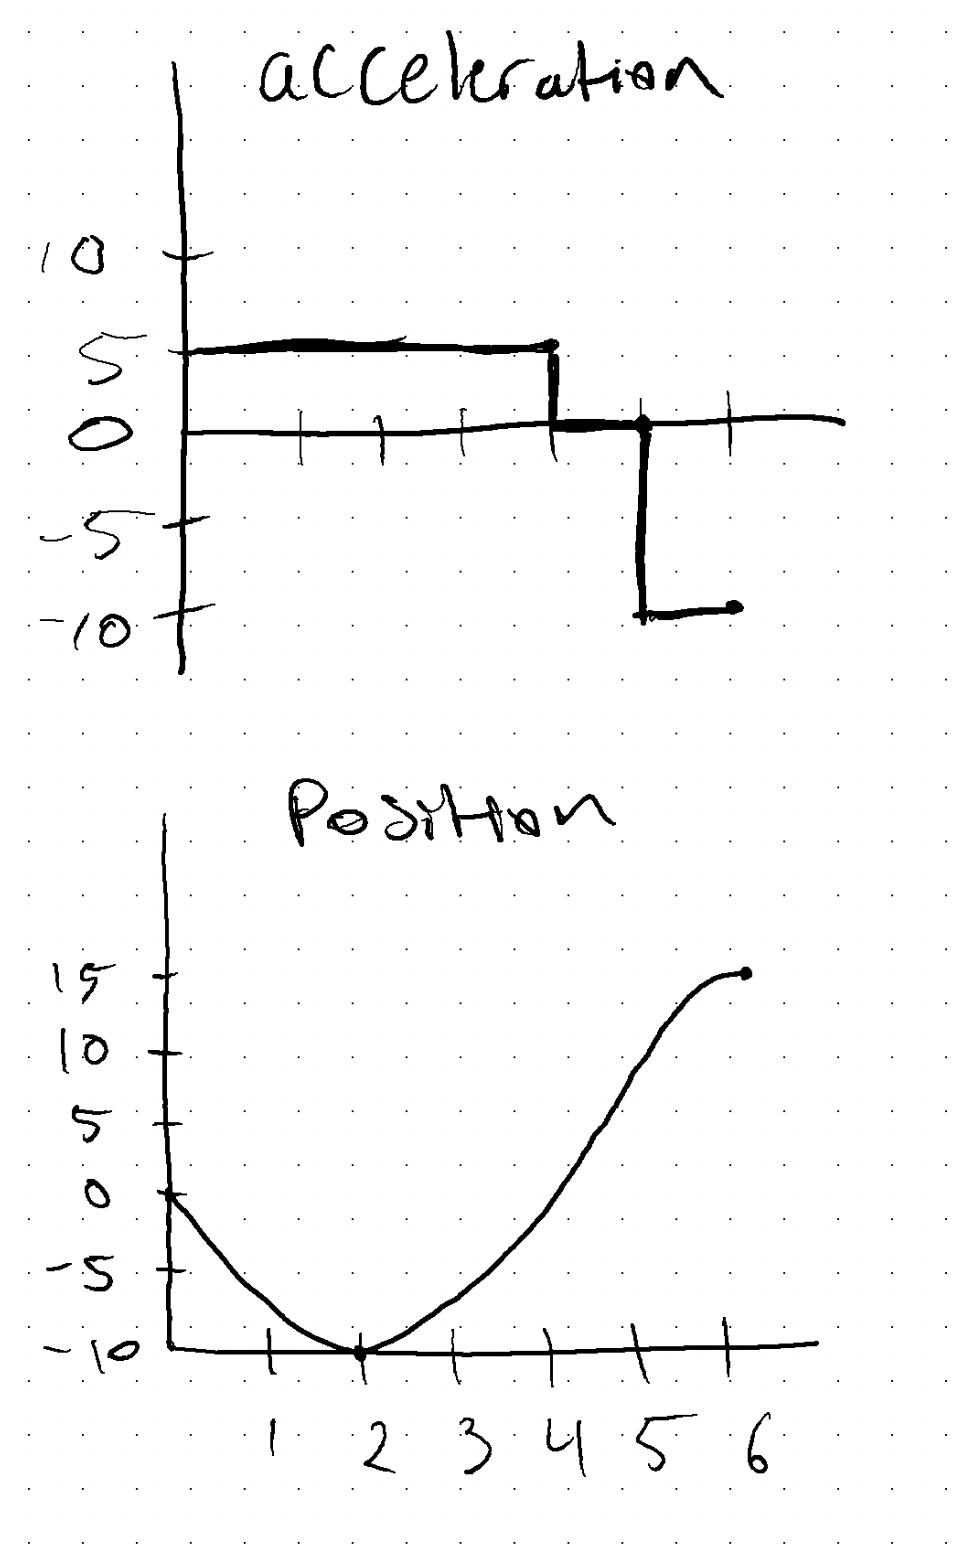
\includegraphics[scale=0.25]{solution-7.png}
\end{figure}


\section*{Problem 8}
The length of a train is 44.5 m. Its front is 100.0 m from a pole. It accelerates from rest at $0.500\ \unit{\meter\per\second^2}$. (a) How long does it take to go past the pole? (b) At what speeds do its front and rear pass the pole?

\subsection*{Solution}

\subsubsection*{Part a:}
To find the time it takes for the front of the train to reach the pole, we use the kinematic equation:
\[
    \Delta x = v_0 t + \frac{1}{2} a t^2
\]
where $\Delta x = 100.0\ \unit{\meter}$, $v_0 = 0$, and $a = 0.500\ \unit{\meter\per\second^2}$. Substituting the values:
\[
    100.0 = 0 + \frac{1}{2}(0.500)t^2
\]
\[
    100.0 = 0.250 t^2
\]
\[
    t^2 = \frac{100.0}{0.250} = 400.0
\]
\[
    t = \sqrt{400.0} = 20.0\ \unit{\second}
\]

\subsubsection*{Part b:}
To find the speed of the front of the train as it passes the pole, we use the equation:
\[
    v = v_0 + at
\]
Substituting $v_0 = 0$, $a = 0.500\ \unit{\meter\per\second^2}$, and $t = 20.0\ \unit{\second}$:
\[
	v = 0 + (0.500)(20.0) = 10.0\ \unit{{\meter\per\second}}
\]
To find the time when the rear of the train passes the pole, we need to calculate how long it takes for the rear to travel an additional 44.5 m (the length of the train).
\[
    \Delta x = v_0 t + \frac{1}{2} a t^2
\]
where $\Delta x = 44.5\ \unit{\meter}$, $v_0 = 10.0\ \unit{\meter\per\second}$, and $a = 0.500\ \unit{\meter\per\second^2}$. Substituting:
\[
    44.5 = (10.0)t + \frac{1}{2}(0.500)t^2
\]
\[
    44.5 = 10.0t + 0.250t^2
\]
Using the quadratic formula:

\[
    t = \frac{-10.0 \pm \sqrt{(10.0)^2 - 4(0.250)(-44.5)}}{2(0.250)}
\]
\[
    t = \frac{-10.0 \pm \sqrt{100.0 + 44.5}}{0.500}
\]
\[
    t = \frac{-10.0 \pm \sqrt{144.5}}{0.500}
\]
\[
    t = \frac{-10.0 \pm 12.02}{0.500}
\]
Taking the positive root:

\[
    t = \frac{-10.0 + 12.02}{0.500} = \frac{2.02}{0.500} = 4.04\ \unit{\second}
\]
Now, to find the speed of the rear of the train as it passes the pole, we use the equation:
\[
    v = v_0 + at
\]
\[
v = 10.0 + (0.500)(4.04) = 10.0 + 2.02 = 12.02\ \unit{{\meter\per\second}}
\]


\end{document}
